% calculus:x22 GDC:YES
\begin{question}
  \hspace*{\fill} [Note maximale: 14]\par
  \noindent On considère $f(x) = x\ln(4 - x^2)$, avec $-2 < x < 2$.\par
  \medskip
  \begin{center}
    \noindent Une partie de la représentation graphique de $f$ est donnée ci-dessous.\par
    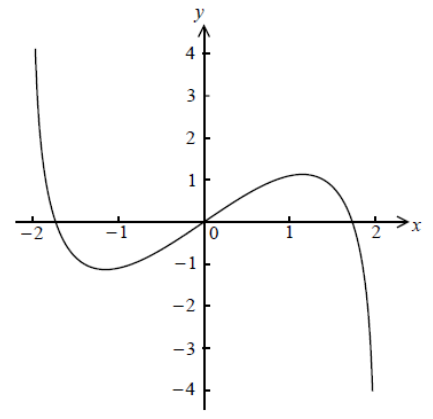
\includegraphics[scale=0.25]{xln4minuxsqr}\par
  \end{center}\par
  (a) Soient $P$ et $Q$ les points de la courbe représentant $f$\par
  \hspace{1em} où la tangente à la représentante graphique de $f$ est parallèle à l'axe des abscisses.\par
  \hspace{1em} (i ) Trouvez l'abscisse de $p$ et $q$.\par 
  \hspace{1em} (ii) On considère $f(x) =k$.\par
  \hspace{3em} Donnez toutes les valeurs de $k$ pour les-quelles il y a exactement deux solutions.\hspace*{\fill} [5]\par
  \medskip
  Soit $g(x) = x^3\ln(4 - x^2)$, avec $-2 < x < 2$.\par
  \medskip
  (b) Montrez que $g^\prime(x)=\frac{-2x^4}{4 - x^2} + 3x^2\ln(4 - x^2)$.\hspace*{\fill} [4]\par
  \medskip
  (c) Esquissez la représentation graphique de $g^\prime$.\hspace*{\fill} [2]\par
  \medskip
  (d) On considére $g^\prime(x) = w$.\par
  \hspace{1em} Donnez toutes les valeurs de $w$ pour les-quelles il y a exactement deux solutions.\hspace*{\fill} [3]\par
  
\end{question}
